\documentclass[10pt]{article}
\usepackage{icmlko}

\icmlmeta{IP 파운데이션 월드모델}{208}{나눗셈은 터지고 셈은 기운다}{노트 207의 아티팩트가 다른 축에도 있나 훑었다. 분모에 시간이 든 축은 둘뿐인데, 시간을 담는 축은 훨씬 많았다 --- 그리고 그것들은 해가 없다}

\begin{document}

\twocolumn[
\icmlheader

\begin{abstract}
노트 207이 웹툰 \texttt{goods\_scale} 의 분모에 긁은 날이 박혀 있는 것을
잡고 ``다른 축에도 분모에 시간이 있나''를 남겼다. 축 파일의 \texttt{why} 를
열 도메인 $\times$ 다섯 축으로 훑었다 --- 자료를 안 건드리고 문서만 읽는
검사다. \textbf{비율이면서 시간말이 든 축은 둘뿐이다} --- 웹툰과 만화의
\texttt{goods\_scale}, 둘 다 노트 207이 다룬 것. \textbf{훑기는 깨끗하다.}
그런데 훑다가 다른 것이 보였다. \texttt{venue\_prominence} 가 일곱
도메인에서 ``\emph{표본 내} 사전 출시작 수''인데, \textbf{표본이 시간으로
잘려 있으므로 늦게 나온 레코드일수록 셀 수 있는 앞선 작품이 많다.} 쟀다 ---
시작 연도와의 상관이 애니 \textbf{$+$0.424} · 펀딩 $+$0.354 · 웹툰 $+$0.295
· 세계애니 $+$0.181 · 모바일 $+$0.165 로 \textbf{일곱 중 다섯}이
$|r|{>}0.15$ 다. 연도를 통제하면 웹툰의 라벨 상관이 $-$0.063 에서
\textbf{$+$0.061} 로 뒤집히고 펀딩은 $-$0.097 에서 $+$0.014 로 사라진다.
\textbf{같은 종류의 오염이다.} 고쳤다 --- 시작 연도 안에서 순위를 다시
매긴다. \textbf{판이 안 움직인다} --- F6 $+$0.0002 · F21 $+$0.0008 · F18
$-$0.0028 로 전부 $|t|{\le}1.6$ 이다. 노트 207의 웹툰 고침이 $+$0.0155
였던 것과 대조된다. \textbf{까닭이 한 줄이다: 나눗셈과 셈은 다르다.}
나눗셈은 분모가 작아질 때 값을 \emph{터뜨린다} --- 웹툰 밀도 중앙이 2018년
0.367 에서 2026년 2.685 로 \textbf{7.3배}다. 셈은 완만히 \emph{기운다} ---
도메인 절편과 순위 정규화가 그 정도는 흡수한다. 그리고 결정적으로 나눗셈
쪽만 유보에서 부호가 뒤집혔다(노트 206의 셋 중 하나). \textbf{그러니 노트
207의 아티팩트는 ``비율이고 분모에 측정 시각이 있다''는 좁은 조건에서만
위험하다} --- 시간을 담는 축은 더 있지만 셈꼴이라 해가 없다.
\end{abstract}
]

\begin{figure*}[t]
\centering
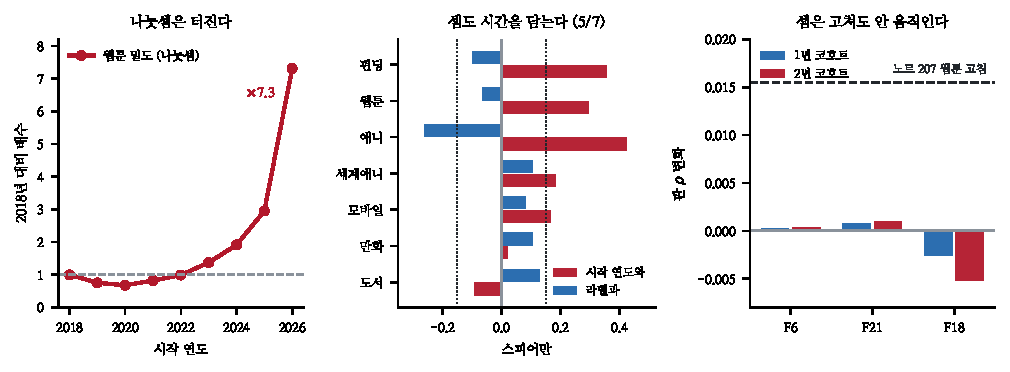
\includegraphics[width=\textwidth]{figs/divide.pdf}
\caption{왼쪽 --- 나눗셈은 터진다. 가운데 --- 셈도 시간을 담는다.
오른쪽 --- 셈은 고쳐도 안 움직인다.}
\end{figure*}

\section{훑기는 깨끗하다}

\begin{table}[t]
\centering\tsize
\caption{축 파일 \texttt{why} 를 열 도메인 $\times$ 다섯 축으로.}
\begin{tabular}{lr}
\toprule
훑은 도메인$\times$축 & 45 \\
비율 꼴 & 3 \\
시간말이 든 것 & 6 \\
\textbf{둘 다} & \textbf{2} \\
\midrule
\multicolumn{2}{l}{웹툰 \texttt{goods\_scale} --- ``연재 밀도 15화/9주''} \\
\multicolumn{2}{l}{만화 \texttt{goods\_scale} --- ``연재 밀도 232화/399주''} \\
\bottomrule
\end{tabular}
\end{table}

\claimx{\textbf{둘 다 노트 207이 이미 다룬 것이다.} 자료를 안 건드리고
문서만 읽는 검사인데 새것이 안 나왔다.}{\textbf{그래도 값이 있는 검사다} ---
안 나왔다는 것을 알아야 다음으로 넘어간다. 그리고 웹툰의 실제 예가
``6화/1주''인 것을 보면 아티팩트가 얼마나 극단인지 바로 보인다.}

\section{셈도 시간을 담는다}

\begin{table}[t]
\centering\tsize
\caption{\texttt{venue\_prominence} $=$ 표본 내 사전 출시작 수.}
\begin{tabular}{lrrr}
\toprule
& 시작 연도와 & 라벨과 & 연도 통제 뒤 \\
\midrule
\textbf{애니} & \textbf{$+$.424} & $-$.261 & $-$.220 \\
\textbf{펀딩} & \textbf{$+$.354} & $-$.097 & \textbf{$+$.014} \\
\textbf{웹툰} & \textbf{$+$.295} & $-$.063 & \textbf{$+$.061} \\
세계애니 & $+$.181 & $+$.106 & $+$.103 \\
모바일 & $+$.165 & $+$.082 & $+$.083 \\
만화 & $+$.022 & $+$.103 & $+$.103 \\
도서 & $-$.093 & $+$.127 & $+$.036 \\
\bottomrule
\end{tabular}
\end{table}

\claimx{\textbf{일곱 중 다섯이 시작 연도와 붙는다.} 표본이 시간으로 잘려
있으니 당연하다 --- 2015년 레코드는 셀 수 있는 앞선 작품이 없고 2024년
레코드는 9년치가 있다.}{웹툰과 펀딩은 통제하면 라벨 상관이 사라지거나
뒤집힌다 --- \textbf{그 축이 재던 것의 절반이 ``언제 나왔나''였다.}}

\section{그런데 고쳐도 안 움직인다}

\begin{table}[t]
\centering\tsize
\caption{시작 연도 안에서 순위를 다시 매기면.}
\begin{tabular}{lrrl}
\toprule
& 1년 코호트 & 2년 코호트 & \\
\midrule
F6 능형 & $+$.0002 & $+$.0003 & $t{\le}0.7$ \\
F21 & $+$.0008 & $+$.0010 & $t{\le}1.6$ \\
F18 배깅 & $-$.0028 & $-$.0052 & $t{\ge}-1.6$ \\
\midrule
\multicolumn{2}{l}{(견줌: 노트 207 웹툰 고침)} & \textbf{$+$.0155} & \\
\bottomrule
\end{tabular}
\end{table}

\claimx{\textbf{예측이 맞았다} --- ``고쳐도 크게 안 움직일 것''을 적었고
$|t|{\le}1.6$ 이다. 걸어 둔 반대 가능성(``상관이 0 이면 축이 멀쩡하다'')은
틀렸다 --- 상관은 있는데 해가 없다.}{\textbf{오염이 있다는 것과 해가
있다는 것이 다르다} --- 노트 179가 ``틀린 값은 이미 죽어 있었다''로 세운
자리와 같은 모양이다.}

\section{나눗셈과 셈}

\claimx{\textbf{나눗셈은 터진다.} 웹툰 밀도 중앙이 2018년 0.367 에서 2026년
2.685 로 \textbf{7.3배}다 --- 분모가 418주에서 8주로 줄었기 때문이다.
값의 \emph{눈금} 자체가 바뀐다.}{\textbf{셈은 기운다.} 사전 작품 수는
코호트마다 조금씩 늘 뿐이고, 도메인 절편과 순위 정규화가 그 정도는
흡수한다.}

\claimx{\textbf{그리고 나눗셈 쪽만 부호가 뒤집혔다.} 노트 206이 잰 부호
뒤집힘 셋에 \texttt{venue\_prominence} 는 없다.}{순위 정규화가 단조
변환에 불변이라 ``완만한 기울기''는 지워지고 ``눈금 폭발''은 안 지워진다
--- \textbf{순위로 바꿔도 코호트 사이의 순서는 남는다.}}

\claimx{\textbf{그러니 검사를 좁힐 수 있다.} ``비율이고 분모에 측정 시각이
있는가'' 하나만 보면 된다 --- 그 조건에 맞는 축은 이 판에 둘뿐이고 둘 다
고쳤다.}{시간을 담는 축은 더 있지만 셈꼴이라 놔둔다. \textbf{고칠 것이
없다는 것도 결과다.}}

\begin{table}[t]
\centering\tsize
\caption{남은 것.}
\begin{tabular}{ll}
\toprule
애니 & 장소 노출이 연도와 $+$0.42 --- 제일 심한데 통제해도 남는다 \\
\textbf{다음 갈래} & 축 정의 말고 --- 라벨 정의로 \\
문서 검사 & 45칸을 손으로 읽었다 --- 자동화할 것인가 \\
\bottomrule
\end{tabular}
\end{table}

두 번째 줄이 다음이다. 이 흐름은 노트 207$\sim$208 에서 \emph{축}의 정의에
측정 시각이 들었는지 봤다. \textbf{라벨은 안 봤다.} 웹툰 라벨은 네이버
즐겨찾기 누적이고 애니는 분기 시청이며 세계애니는 누적 회원이다 ---
\textbf{누적 라벨은 정의상 오래된 레코드에 유리하다.} 노트 181이 ``애니
라벨은 속편을 벌하고 세계애니 라벨은 안 벌한다''를 쟀는데 그것도 누적이냐
분기냐의 차이였다. \textbf{라벨에도 같은 검사를 대면 축보다 큰 것이 나올 수
있다} --- 축은 다섯 칸이고 라벨은 도메인마다 하나뿐이라 잘못되면 그 도메인
전체가 흔들린다.

\end{document}
